\chapter{Results}
In this chapter, we will present some results obtained during the project. Including inference examples and predictions performed on the tiles of the Cantabria dataset. We will also describe the post‑processing procedures applied to the model’s outputs, and finally, determine the intersection region between the vegetation and the high-voltage power lines.\\

\section{Inference examples} 
We begin by visualizing a set of inference examples. We have selected three images, each originating from one of the previously mentioned datasets. Predictions were then performed on these images using two models, one trained on the Jordan Forests Dataset and another trained on the LoveDA Dataset. 
\begin{figure}[H]
\centering
\begin{subfigure}{0.32\textwidth}
    \centering
    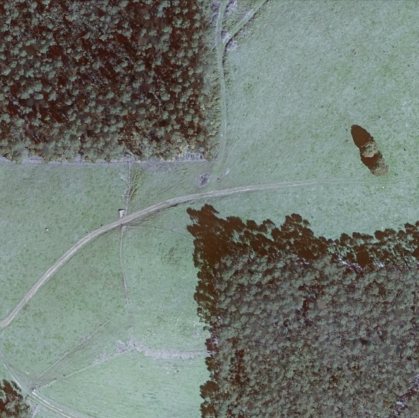
\includegraphics[width=\textwidth]{IMAGENES/Result_Img1.png}
    \caption{Cantabria Image}
    \label{fig:img1}
\end{subfigure}
\hfill
\begin{subfigure}{0.32\textwidth}
    \centering
    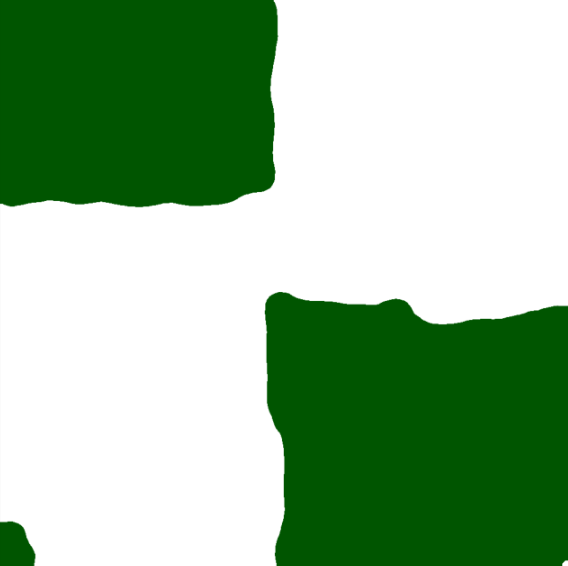
\includegraphics[width=\textwidth]{IMAGENES/Result_Mask1_J.png}
    \caption{Mask (Jordan Forests Model)}
    \label{fig:img2}
\end{subfigure}
\hfill
\begin{subfigure}{0.32\textwidth}
    \centering
    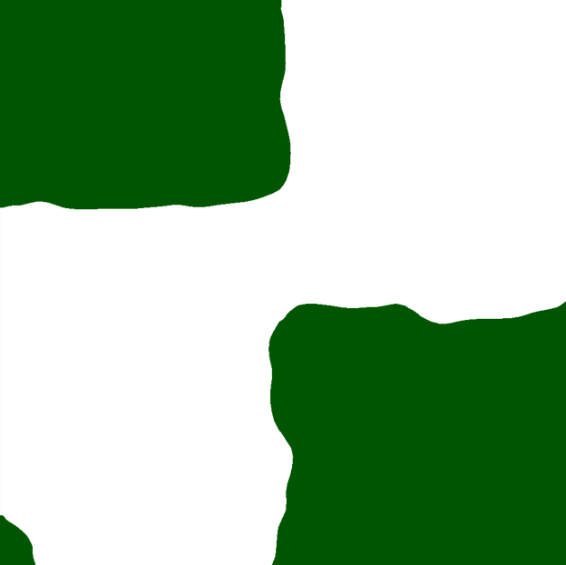
\includegraphics[width=\textwidth]{IMAGENES/Result_Mask1_Lo.png}
    \caption{Mask (LoveDA Model)}
    \label{fig:img3}
\end{subfigure}
\begin{subfigure}{0.32\textwidth}
    \centering
    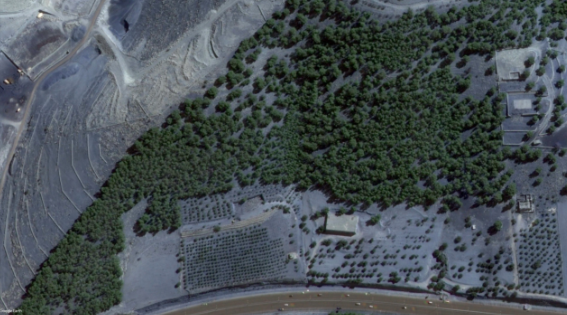
\includegraphics[width=\textwidth]{IMAGENES/Result_Img2.png}
    \caption{Jordan Forests Image}
    \label{fig:img1}
\end{subfigure}
\hfill
\begin{subfigure}{0.32\textwidth}
    \centering
    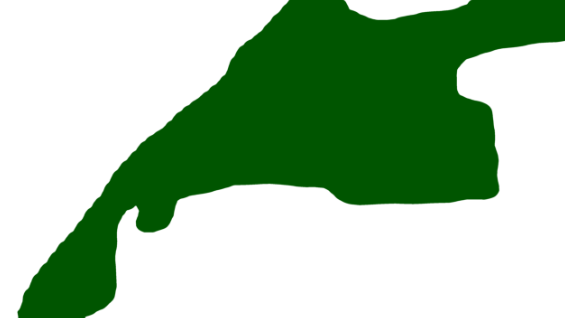
\includegraphics[width=\textwidth]{IMAGENES/Result_Mask2_J.png}
    \caption{Mask (Jordan Forests Model)}
    \label{fig:img2}
\end{subfigure}
\hfill
\begin{subfigure}{0.32\textwidth}
    \centering
    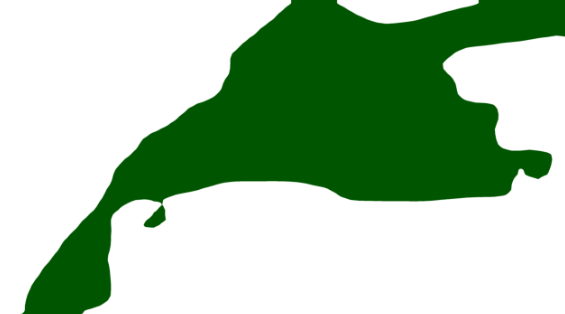
\includegraphics[width=\textwidth]{IMAGENES/Result_Mask2_Lo.png}
    \caption{Mask (LoveDA Model)}
    \label{fig:img3}
\end{subfigure}
\begin{subfigure}{0.32\textwidth}
    \centering
    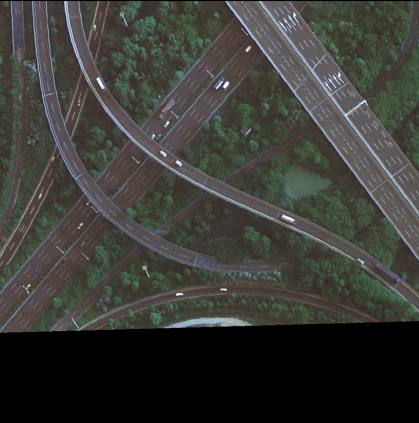
\includegraphics[width=\textwidth]{IMAGENES/Result_Img3.png}
    \caption{LoveDA Image}
    \label{fig:img1}
\end{subfigure}
\hfill
\begin{subfigure}{0.32\textwidth}
    \centering
    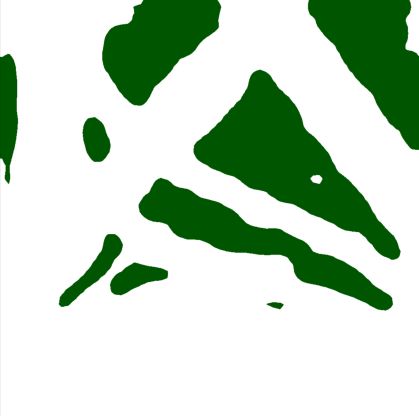
\includegraphics[width=\textwidth]{IMAGENES/Result_Mask3_J.png}
    \caption{Mask (Jordan Forests Model)}
    \label{fig:img2}
\end{subfigure}
\hfill
\begin{subfigure}{0.32\textwidth}
    \centering
    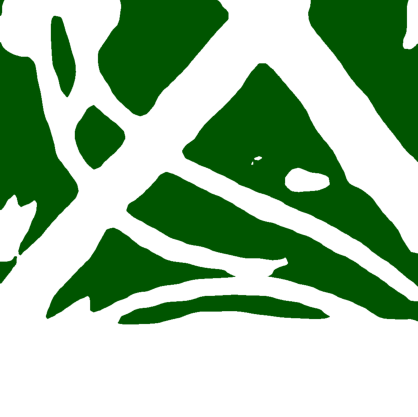
\includegraphics[width=\textwidth]{IMAGENES/Result_Mask3_Lo.png}
    \caption{Mask (LoveDA Model)}
    \label{fig:img3}
\end{subfigure}
\caption{Examples of predictions on different images using 2 models, one trained on LoveDA Dataset and another one trained on Jordan Forests Dataset.}
\label{fig:combined}
\end{figure}


As illustrated in the Figure 5.1, each model achieves good predictive results on images from its corresponding training set. However, the Jordan Forests model demonstrates poor performance on the selected LoveDA image. This limitation is because the Jordan Forests Dataset is mainly consisted of forest images, which concedes the model the ability to detect large forested areas but leaves it less effective at identifying smaller vegetation regions. In the case of the Cantabria image, both models achieved similar performance on the selected example. Nevertheless, after evaluating other images within the Cantabria dataset, we observed that the LoveDA models are more effective at capturing forest edges and smaller vegetation regions, whereas the Jordan models perform better when detecting extensive forested areas. 

\section{Inference on Cantabria dataset (Tiles)}
\subsection{Inference process}
Next, we will describe the inference process on the tiles exported during the Data Preparation stage, which differs slightly from the inference process on smaller images.


\begin{figure}[H]
 \centering
 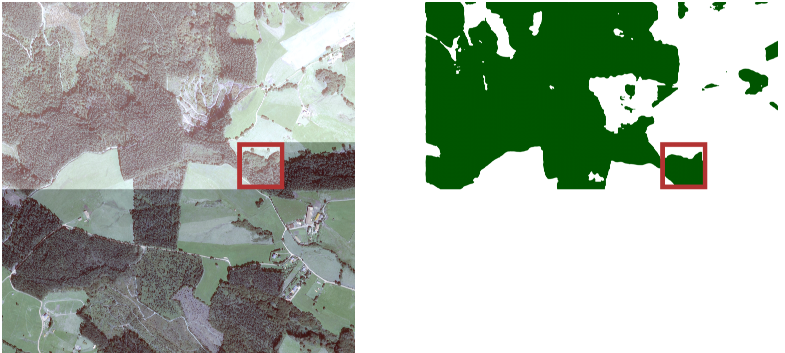
\includegraphics[scale=0.75]{IMAGENES/IMG17-Inference-process.png}
 \captionsetup{font=large}
 \caption {Inference process on Cantabria dataset. The model acts as a "sliding window" that scans over a large tile. The size of the window is 1000 x 1000 pixels.}
\end{figure}

 As previously mentioned, each tile has dimensions of 15000 x 15000 pixels, which is a very large input and therefore cannot be passed directly to the model. To perform the inference, we first loaded the entire tile into the training framework, then divided it into smaller sub-tiles of 1000 x 1000 pixels. Each sub-tile was subsequently fed into the model for prediction.  This process can be seen as using the model as a "sliding window" that scans over a large image and constructing the final mask by merging the predictions of all sub-tiles. 

\newpage


\subsection{Sharp Transitions}

The prediction mask obtained from the inference on one of the tiles is shown in the figure below: 

 \begin{figure}[H]
\centering
\begin{subfigure}{0.49\textwidth}
\centering
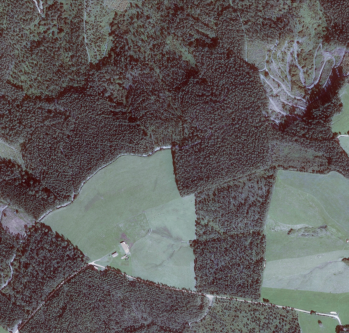
\includegraphics[width = \textwidth]{IMAGENES/IMG18-No-Aver-Img.PNG}
\caption{Cantabria dataset (Image)}
\label{fig:left}
\end{subfigure}
\begin{subfigure}{0.50\textwidth}
\centering
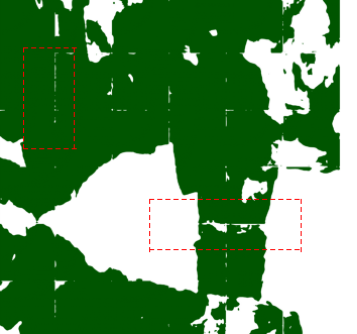
\includegraphics[width = \textwidth]{IMAGENES/IMG18-No-Aver-Mask2.PNG}
\caption{Cantabria dataset (Mask)}
\label{fig:right}
\end{subfigure}
\caption{Prediction on one of the tiles of Cantabria dataset. Dashed red rectangles highlight the regions where there are sharp transitions in the mask, these areas correspond to the junction regions between the sub-tiles.}
\label{fig:combined}
\end{figure}

As observed, there are multiple regions with sharp transition in the prediction mask, these regions align with the junction between the sub-tiles, which indicates that the model tends to perform poorly near the sub-tile boundary. One of the main reasons for this issue is that the model relies on surrounding pixels to make prediction on the target pixel. Therefore, when a forested area is divided across two sub-tiles, and one tile contains only a small fragment of the forest along its edge, it becomes difficult for the model to correctly classify these border pixels as forest. 
\newpage

\subsection{Solution}
To address this problem, one approach is to perform additional inferences on the junction regions between sub-tiles. Therefore, instead of relying on a single inference per sub-tile, 5 inferences were performed, 4 at the corners and 1 at the center.

\begin{figure}[H]
 \centering
 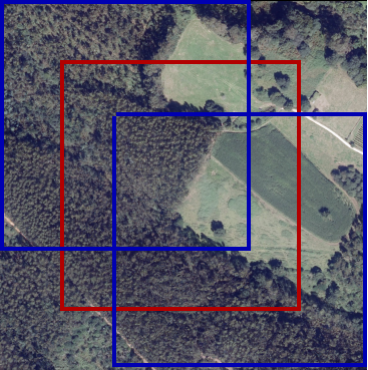
\includegraphics[scale=0.75]{IMAGENES/IMG19-Multi-inference.png}
 \captionsetup{font=large}
 \caption {Additional inferences. The red rectangle marks the target sub-tile where the prediction will be applied. For each sub-tile, 4 inferences were performed at the corners (for simplicity, this figure shows only 2 additional inferences, blue rectangles), and 1 inference was performed at the center (red rectangle).}
\end{figure}

 The corner inferences cover a subsection of the target sub-tile as well as parts from adjacent sub-tiles, providing additional contextual information to improve border pixels classification. Finally, all the inference results are averaged to produce the final output mask. The results obtained by using this approach are shown in the figure below: 
\newpage


\begin{figure}[H]
\centering
\begin{subfigure}{0.49\textwidth}
\centering
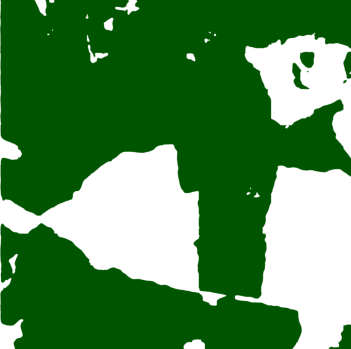
\includegraphics[width = \textwidth]{IMAGENES/IMG20-Aver-Mask.png}
\caption{Prediction mask with additional inferences.}
\label{fig:left}
\end{subfigure}
\begin{subfigure}{0.49\textwidth}
\centering
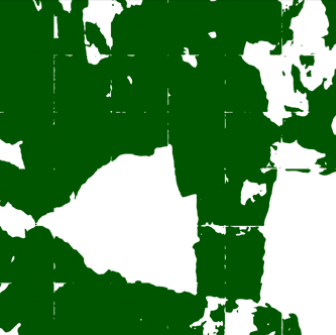
\includegraphics[width = \textwidth]{IMAGENES/IMG18-No-Aver-Mask.png}
\caption{Prediction mask without additional inferences.}
\label{fig:right}
\end{subfigure}
\caption{Comparison between the prediction with and without averaging.}
\label{fig:combined}
\end{figure}

As shown, there is a significant improvement in the prediction mask, particularly along the borders of the sub-tiles where sharp transitions were previously visible. Additionally, since the final mask is obtained by averaging the results from multiple inferences, there is also an increase in the prediction accuracy.\\


\section{Postprocessing}

In order to determine the intersection areas between the vegetation and power lines, the masks obtained from the previous section must be further processed. This postprocessing step included adding georeferencing information and converting the masks into a more suitable format to simplify the calculation of intersection areas.\\

The georeferencing was performed by using a Python script with the GDAL library, which merged each mask with its corresponding georeferencing file and converted it from PNG to GeoTIFF (a georeferenced raster image). Regarding the mask conversion, one option considered during the project was to transform the raster masks into tables of coordinates. In other words, each vegetation pixel would be converted into its corresponding latitude and longitude values and stored as a vector. These vegetation coordinates could then be loaded alongside the power line data, and the intersections were determined by using functions from GeoPandas library.\\

However, storing pixel level coordinates presented a significant drawback, which is that the computation time for intersection detection was extremely long due to the large number of pixels involved, because the algorithm needed to scan every pixel and evaluate whether it intersected with the power line data. Therefore, to accelerate processing time, an alternative approach was adopted: Instead of converting all vegetation pixels into coordinates, only the contour coordinates of each vegetation object in the prediction mask were extracted and stored.\\

 \begin{figure}[H]
\centering
\begin{subfigure}{0.49\textwidth}
\centering
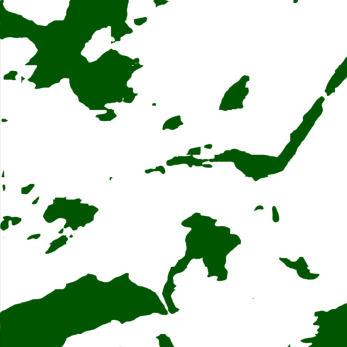
\includegraphics[width = \textwidth]{IMAGENES/IMG21-Contour1.png}
\caption{Prediction mask.}
\label{fig:left}
\end{subfigure}
\begin{subfigure}{0.49\textwidth}
\centering
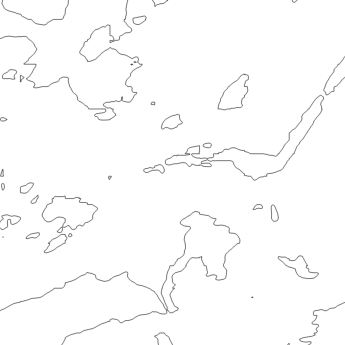
\includegraphics[width = \textwidth]{IMAGENES/IMG21-Contour2.png}
\caption{Contours of vegetation objects.}
\label{fig:right}
\end{subfigure}
\begin{subfigure}{0.60\textwidth}
\centering
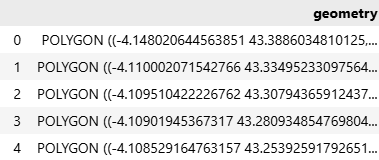
\includegraphics[width = \textwidth]{IMAGENES/IMG21-Contour3.png}
\caption{Contours stored as geometry objects.}
\label{fig:right}
\end{subfigure}
\caption{(a)->(b)->(c) shows the process of converting prediction mask into coordinates.}
\label{fig:combined}
\end{figure}

The contours extraction was achieved by using a function from the OpenCV library, which detects contours of each object in binary images based on the algorithm proposed in this paper [26]. Once extracted, the contour coordinates were converted into geometry objects (commonly used format for handling geospatial data) using the Shapely library. These objects are represented as text strings (Figure 5.6.c) that contain coordinate information, preceded by a header that specifies the geometry type (for vegetation objects, the extracted contours were stored specifically as polygons), and the GeoPandas library can directly parse and interpret this format. 


\section{Intersection with power line}
After converting the prediction masks into coordinates and saving them as geometry objects, these were combined with the power line data to determine the intersection areas. To ensure compatibility, the power line dataset was also converted into geometry objects, stored specifically as StringLines. \\

Since the aim of the projects was to identify potential contact regions rather than exact contact points, a buffering step was applied to the power line geometries. This buffer expanded the lines by a given margin, creating a zone that represents the potential contact area (see figure below). And every vegetation polygon falling inside this buffered zone was flagged as a risk zone. 

\begin{figure}[H]
 \centering
 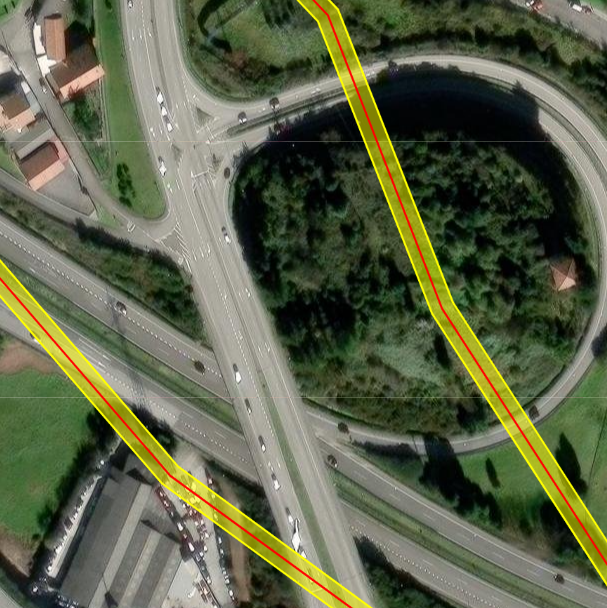
\includegraphics[scale=0.49]{IMAGENES/IMG22-PowerLine2.png}
 \captionsetup{font=large}
 \caption {Power line data. The red lines represent the power line coordinates, and the yellow zones correspond to the buffer.}
\end{figure}

Some examples of the intersection areas are shown in the figure below: 

 \begin{figure}[H]
\centering
\begin{subfigure}{0.32\textwidth}
\centering
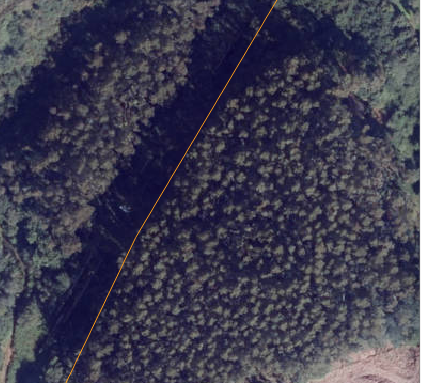
\includegraphics[width = \textwidth]{IMAGENES/Intersection1.png}
\caption{Raster image.}
\label{fig:left}
\end{subfigure}
\begin{subfigure}{0.328\textwidth}
\centering
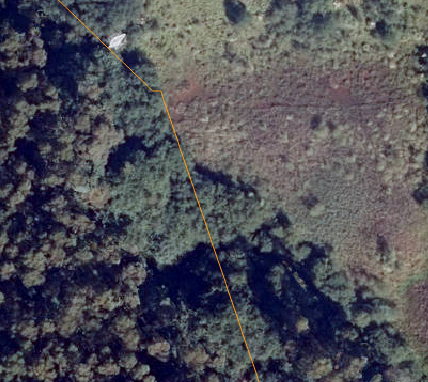
\includegraphics[width = \textwidth]{IMAGENES/Intersection2.png}
\caption{Raster image.}
\label{fig:right}
\end{subfigure}
\begin{subfigure}{0.305\textwidth}
\centering
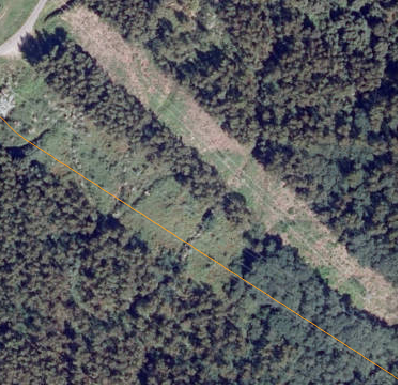
\includegraphics[width = \textwidth]{IMAGENES/Intersection3.png}
\caption{Raster image.}
\label{fig:left}
\end{subfigure}
\begin{subfigure}{0.31\textwidth}
\centering
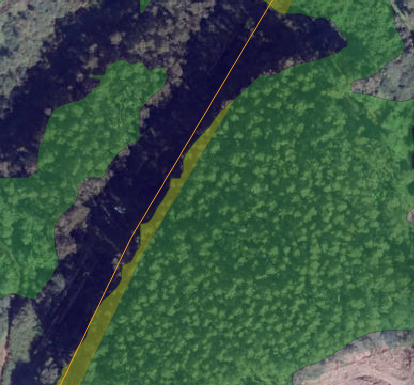
\includegraphics[width = \textwidth]{IMAGENES/Intersection1-m.png}
\caption{Intersection areas for figure (a).}
\label{fig:right}
\end{subfigure}
\begin{subfigure}{0.33\textwidth}
\centering
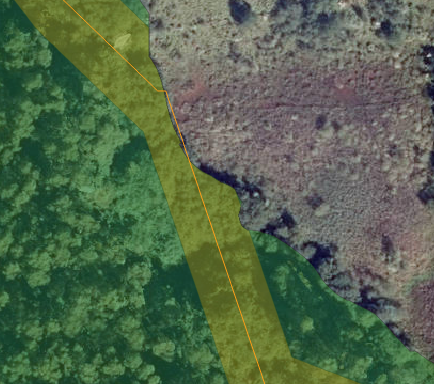
\includegraphics[width = \textwidth]{IMAGENES/Intersection2-m.png}
\caption{Intersection areas for figure (b).}
\label{fig:right}
\end{subfigure}
\begin{subfigure}{0.31\textwidth}
\centering
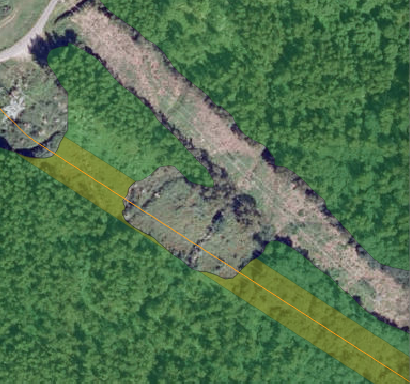
\includegraphics[width = \textwidth]{IMAGENES/Intersection3-m.png}
\caption{Intersection areas for figure (c).}
\label{fig:left}
\end{subfigure}
\caption{Examples of intersection areas. }
\label{fig:combined}
\end{figure}

As illustrated, several risk zones were detected where potential contact between power lines and vegetation could occur. In certain regions, the power lines do not actually come into contact with the trees (Figures 5.8.a and 5.8.b), because the utility poles are significantly taller than the surrounding vegetation. However, there are also some other risk zones that appear as a result of misclassified forest pixels (Figure 5.8.c). After evaluating other intersection areas, we have concluded that this degradation in the model performance could be attributed mainly to 2 factors: 

\begin{itemize}
    \item \textbf{Differences in vegetation species}: The models were trained on forest imagery from Jordan and China, but predictions were performed on forests in Cantabria. Thus, the variation in vegetation types across regions could produce distinct textural patterns in satellite imagery. Since the training data may not have included sufficient examples of forest types, the models were less effective in generalizing to Cantabria images, leading to misclassifications. 
    \item \textbf{Image resizing}: As previously mentioned, the input images have been resized to 512 x 512 pixels regardless of their original dimensions in order to reduce memory consumption. However, this resizing process has also led to the loss of fine details due to compression. This is a major drawback because these details are often relevant for pixel-level classification, and working with smaller images increases the difficulty for the model to correctly capture the shape and boundaries of tree canopies.  
\end{itemize}

In conclusion, while the models have identified the majority of vegetation areas, some detected regions present false positives due to certain limitations. Specifically, these limitations stem from insufficient variability in the training data and from transformations applied to the training images as a consequence of the high computational requirements. Although some of these limitations might be unavoidable, several improvements have been considered for a potential future work to improve the accuracy of the vegetation identification and intersection analysis. \\

\section{Future directions}
\begin{itemize}
    \item \textbf{High quality labeled Cantabria dataset}: The most direct way to increase the model performance on Cantabria images is to train the model on the forest images of Cantabria (or similar forested regions in Spain). However, as mentioned before, this is usually a time-consuming task as it requires manual annotation of forested areas.  
    \item \textbf{Pretrained backbone}: The DeeplabV3 models in this project employ a backbone pretrained on the ImageNet-1k dataset, which contains images that are not directly relevant to forest segmentation task. A more suitable strategy would be to use a backbone pretrained on Cantabria forest images, which would allow the model to become “familiar” with the forest species in this region. Furthermore, since the backbone primarily serves as a feature extractor, it can be pretrained using self-supervised learning methods that do not require labeled data. 
    \item \textbf{Exploration of alternative architectures}: In this project, only four architectures were tested. These models can be served as useful benchmarks for comparing other architectures that may achieve superior performance on vegetation segmentation tasks. For instance, transformer-based architectures (SegFormer or Mask2Former) have shown strong performance in recent computer vision research. Additionally, some lightweight architectures optimized for remote sensing could offer a better balance between accuracy and computational efficiency. 
\end{itemize}

 



 




 

 

 






 








